% \section{Modelo usando variables genómicas}

Otra de las preguntas que nos hicimos fue si la consideración de variables genómicas, como medidas de conservación de la posición genómica de la variante, de su entorno, del exón en que se encuentra, la cantidad de variantes observadas en el exón, etc, pueden mejorar el poder predictivo de nuestro modelo. Esta pregunta tiene lugar si consideramos que es en los genes donde se produce la mutación que finalmente da origen a la variante en la proteína. En la base de datos Humsavar existe, para la mayoría de las mutaciones, el identificador rsID o Reference SNP ID. Un identificador rsID agrupa los distintos reportes que hacen referencia a la misma posición dentro del mismo genoma de referencia (hg19/GRCh37, en nuestro caso). A partir de este identificador fue posible obtener de la base de datos dbSNP (Versión snp150) \cite{dbSNP}, datos como el cromosoma, la posición, el cambio de nucleótido de la variante y su clasificación funcional.

\section{Variables de conservación}

En la literatura encontramos que dos de las variables genómicas asociadas a la conservación eran las que daban mejores resultados de predicción (modelos FATHMM-MKL \cite{Shihab2015} y VEST \cite{Carter2013}). La \textit{conservación} es un concepto biológico que refiere a las secuencias conservadas, es decir, secuencias tanto genéticas como proteicas que se mantienen de forma similar o idéntica en muchas especies que poseen un ancestro evolutivo en común. La conservación puede ser cuantificada con distintos tipos de enfoques, pero en lo que nos concierne, dos de los más utilizados son 1) a través de alineamientos múltiples de secuencias, y 2) mediante el uso de árboles filogenéticos.

En particular, la composición de estas variables consiste en alineamientos múltiples de secuencias genéticas (MSA) de 46 especies de vertebrados, incluyendo Homo Sapiens y otras como Felis catus (gato doméstico), Danio renus (pez cebra) y Equus Caballus (caballo). En base a este alineamiento se usan dos medidas distintas que buscan detectar aquellas regiones en el genoma (ADN) con mayor nivel de conservación entre las distintas especies. Las medidas son las siguientes:
\begin{itemize}
    \item \textbf{PhastCons-46-Way}: Medida de conservación basado en un modelo oculto de Markov (\textit{phylo-HMM}). Calcula la probabilidad de que un nucleótido pertenezca a un sitio conservado (considerando el entorno) \cite{siepel2005evolutionarily}.
    \item \textbf{PhyloP-46-Way}: Mide la conservación considerando un alineamiento múltiple y un modelo de evolución neutral. Además, cada columna se mide individualmente, es decir, sin considerar sus columnas vecinas \cite{Pollard2010} 
\end{itemize}

Decidimos incluir en nuestro dataset ambas medidas de conservación, usando el Table Browser de la Universidad de California en Santa Cruz (UCSC) \cite{Karolchik2004}.

\section{Variables relativas a la clase funcional}

También tomamos en consideración la función de la posición dentro del gen. La base de datos dbSNP define cada SNP de acuerdo a su clase funcional. Si la variación se encuentra cerca del intervalo de un transcripto, pero no en la región codificante, la clase funcional va a depender de la posición de la variación relativa a la estructura del transcripto \cite{Kitts2014}.  Por otro lado, si la variación se encuentra en una zona codificante, la clase funcional se va a definir en base a si el alelo de la variación va a resultar en una sustitución sinónima (es decir, el nuevo codón va a formar el mismo aminoácido), una sustitución \textit{missense} (es decir, el nuevo codón va a formar un aminoácido distinto) o una sustitución \textit{nonsense} (en donde la mutación genera un codón de terminación prematuro). En base a esta información generamos variables binarias, que indican con 1 ó 0 la existencia de un lugar con una determinada clase funcional.

Las categorías de clases funcionales que usamos en este caso fueron \cite{tablefuncclasses}:
 
\begin{itemize}
    \setlength\itemsep{0em}
    \item INTRON
    \item MISSENSE
    \item NEAR-GENE
    \item NCRNA
    \item CODING-SYNON
    \item UNTRANSLATED
    \item NONSENSE
    \item SPLICE
    \item STOP-LOSS
\end{itemize}

\section{Extracción de variables usando SNVBox}

Por último, usamos variables genómicas del dataset SNVBox, específicamente de la tabla \\ EXON\_FEATURES. Las variables usadas son:
\begin{itemize}
    \item ExonConservation (CONS): Score de Conservación para el exón completo calculado a partir de una alineación filogenética a 46 vías, usando el \textit{Genome Browser}. Si bien existe una gran similitud con las variables de conservación que ya incluimos en el dataset esta se encuentra a nivel de exón, mientras que las dos variables anteriores se encuentran a nivel de nucleótido. También decidimos incluir esta variable debido a su baja correlación con las mencionadas anteriormente (ver descripción estadística del dataset más adelante).
    \item ExonHapMapSnpDensity (HAPMAP\_SNP\_DEN): Número de SNPs (verificados en HapMap) en el exón donde ocurre la mutación dividido por la longitud del exón. Estos SNPs (también llamados tag SNPs) son los que identifican haplotipos. Los haplotipos son bloques de SNPs heredados por un único individuo.
    \item ExonSnpDensity (SNP\_DEN): Número de SNPs en el exón donde ocurre la mutación dividido por la longitud del exón.
\end{itemize}

Estas variables se definen a nivel de exón, por lo que cada una de ellas posee dos identificadores: UID (identificador de la secuencia proteica a la que pertenece, propia de la base de datos) y EXON ID (identificador del exón dentro de cada transcripto mRNA). Estos identificadores permiten el cruce con la tabla \texttt{Transcript\_Exon} dentro de la base SNVBox (ver figura \ref{fig:exon_diagram}). Con esta tabla podemos obtener el número del cromosoma del exón, y la posición de inicio y fin del exón dentro del cromosoma. Una vez obtenidos estos datos, pudimos extraer todos los rsID dentro de esa subsecuencia. Para aproximadamente el 33\% de los rsIDs en nuestra tabla Humsavar existe más de un transcripto que los contiene, por lo que decidimos promediar las variables (CONS, SNP\_DEN y HAPMAP\_SNP\_DEN) de cada uno de los transcriptos.

\begin{figure}[H]
\centering
    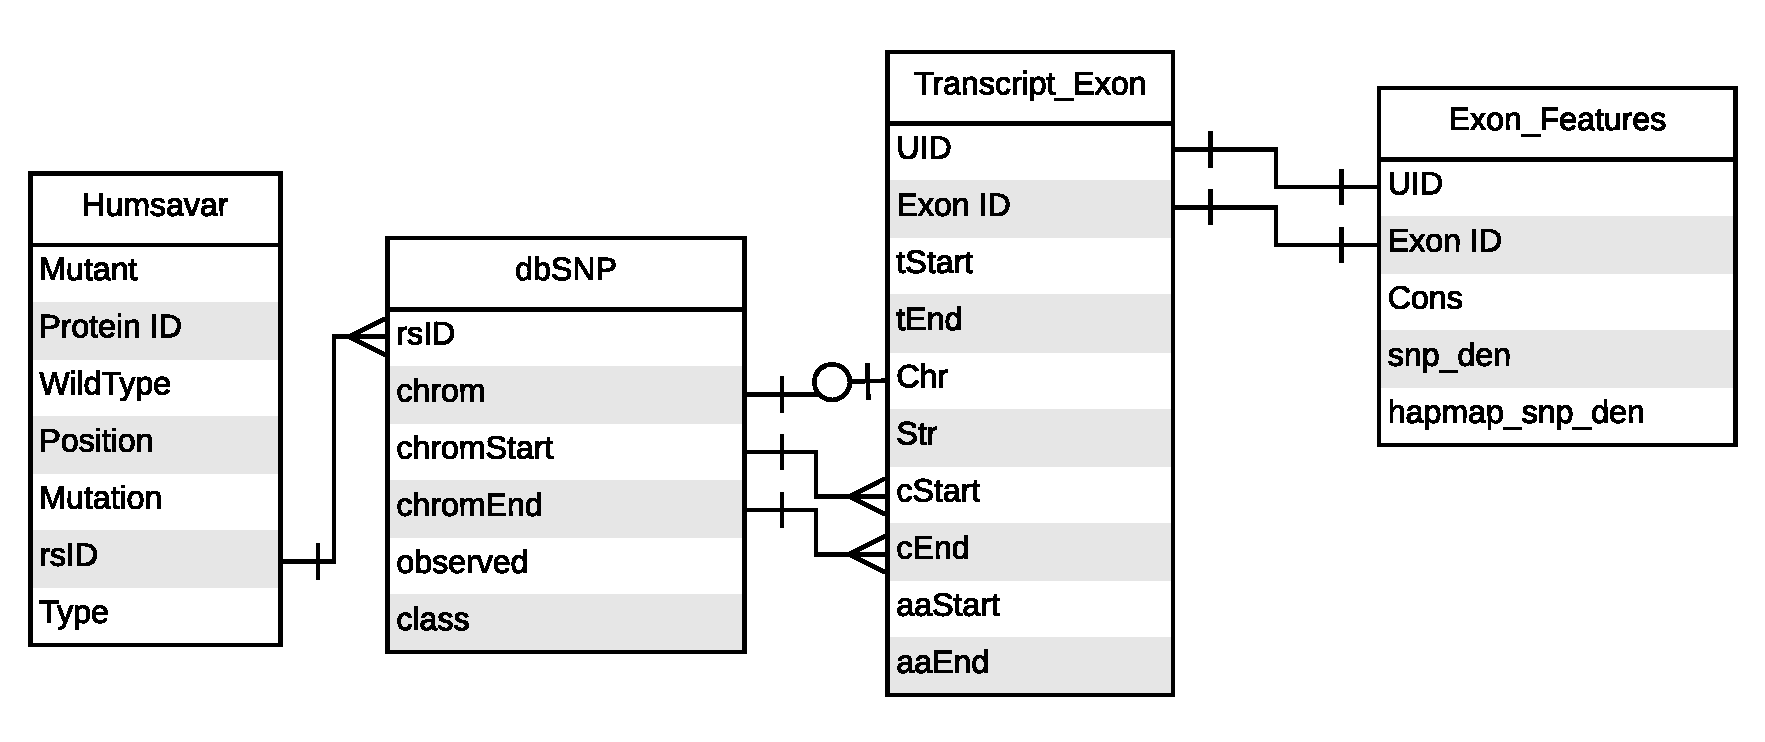
\includegraphics[scale=0.40]{documents/latex/figures/3/genomic/exon_diagram.pdf}
    \caption{Esquema de acceso a las variables genómicas de SNVBox. Las flechas simbolizan la cardinalidad en la relación entre las entidades: uno a muchos (la flecha con 3 puntas), uno a uno (la flecha que une UID con UID, por ejemplo) y uno a opcionalmente uno (chrom a Chr).}
    \label{fig:exon_diagram}
\end{figure}

\section{Construcción del dataset Genómico}

Con los atributos mencionados anteriormente, pudimos cruzar la información usando la columna rsID (Reference SNP cluster ID). Esta columna identifica a un cluster de variaciones de un sólo nucleótido que pertenece a la misma posición en el genoma (o conjunto de posiciones) \cite{Ostell2007}. Filtramos las variantes de Humsavar que no poseían este identificador. Finalmente el dataset Genómico se compone de 55,382 variantes de las cuales 37,572 (68\%) son benignas y 17,807 (32\%) son patogénicas. 

\section{Descripción estadística del dataset Genómico}

A continuación presentamos, como en las secciones anteriores, una descripción de las variables usadas (ver tablas \ref{conservacion_vars} y \ref{snvbox_vars}). Para cada uno de los grupos analizamos la media (mean), el desvío estándar (std), los cuartiles (25\%, 50\%, 75\%) y los valores máximos (max) y mínimos (min). En el caso de la variable de conservación PHASTCONS46WAY encontramos que la mediana y el máximo están muy cercanos (0.99 y 1.00), por lo que podemos anticipar que los valores más interesantes (es decir, aquellos que determinen patogenicidad) se encontraran cerca del mínimo. Algo parecido sucede con la otra variable de conservación, PHYLOP46WAY, donde la mediana, el tercer cuartil y el máximo están mucho más cerca que el resto de los valores.

También calculamos el AUC univariado y el \textit{Balanced Accuracy} para las variables categóricas, en este caso las relativas a la clase funcional. El AUC univariado de las variables de conservación (PHYLOP46WAY, PHASTCONS46WAY y CONS) es alto, lo que significa que variantes en zonas de alta conservación son buenos indicadores de patogenicidad. En el caso de las variables categóricas del dataset (las variables relativas a la clase funcional), no encontramos variables con un BACC significativo.

\newpage

% \subsection{Variables de Conservación}
\begin{table}[H]
\centering
\begin{tabular}{|l|l|l|l|l|l|l|l|l|}
\hline
Variable & mean & std & min & 25\%  & 50\% & 75\%  & max & AUC \\ \hline
PHYLOP46WAY & 2.16 &  2.29 & -8.22 &  0.29 &  1.81 &  4.23 &  6.42 & 0.83 \\ \hline
PHASTCONS46WAY & 0.67 & 0.44 &  0.00 &  0.06 &  0.99 &  1.00 &  1.00 & 0.78 \\ \hline
\end{tabular}
\caption{Variables de Conservación del dataset Genómico.}
\label{conservacion_vars}
\end{table}

% \subsection{}
\begin{table}[H]
\centering
\begin{tabular}{|l|l|l|l|l|l|l|l|l|}
\hline
Variable         & mean & std  & min  & 25\% & 50\% & 75\% & max & AUC  \\ \hline
CONS             & 0.65 & 0.09 & 0.14 & 0.59 & 0.66 & 0.72 & 0.90 & 0.65 \\ \hline
SNP\_DEN         & 0.06 & 0.10 & 0.00 & 0.03 & 0.04 & 0.06 & 1.04 & 0.56 \\ \hline
HAPMAP\_SNP\_DEN & 0.00 & 0.00 & 0.00 & 0.00 & 0.00 & 0.00 & 0.04 & 0.48 \\ \hline
\end{tabular}
\caption{Variables extraídas de SNVBox a nivel de Exón del dataset Genómico.}
\label{snvbox_vars}
\end{table}

% \subsection{Correlación entre las variables}

Con respecto a los valores nulos, tenemos una cobertura muy alta de todas las variables, con un porcentaje de nulos máximo del 2\%. (figura \ref{fig:proporcion_nulos_genomic}). Si consideramos las variantes removidas por no poseer un identificador rsID, este porcentaje aumenta.


% \newpage

\begin{figure}[H]
    \centering
    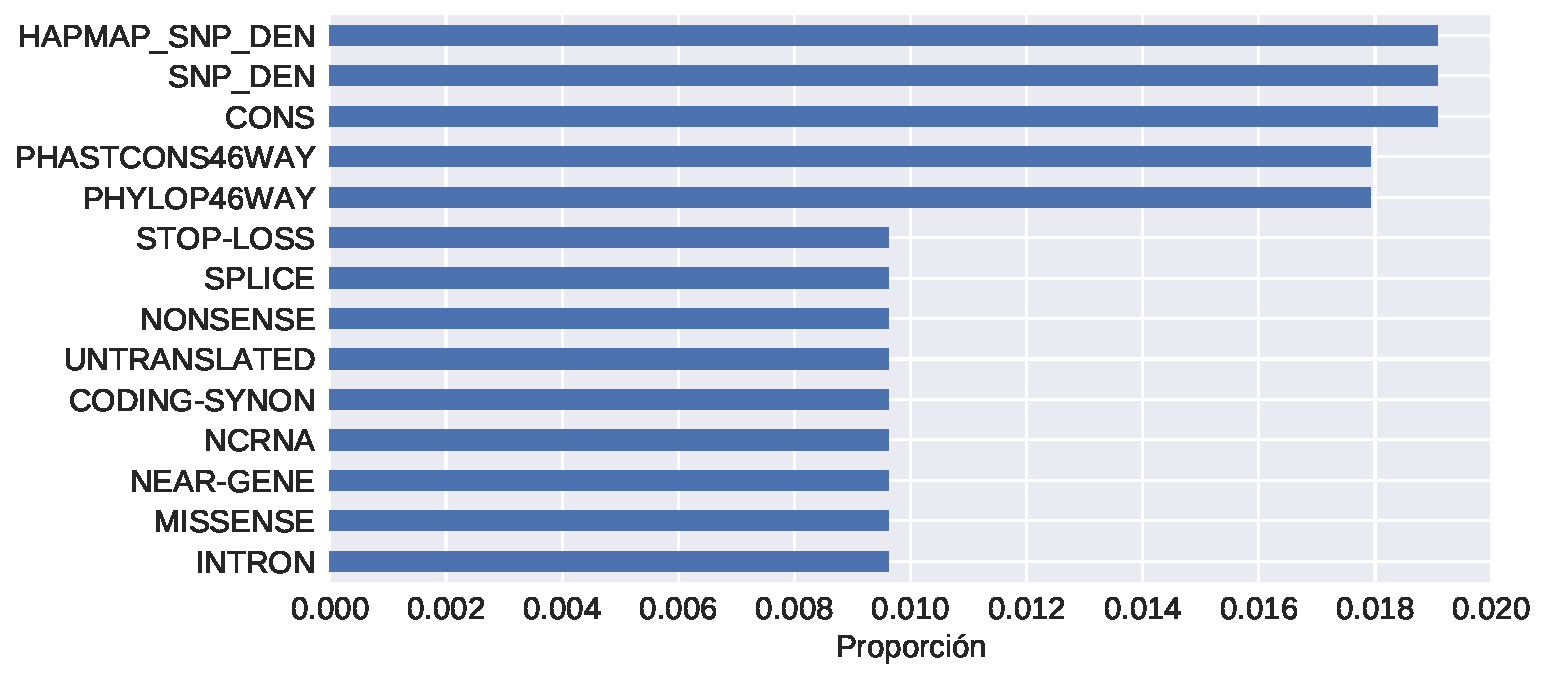
\includegraphics[scale=0.6]{documents/latex/figures/3/genomic/proporcion_nulos_genomic.pdf}
    \caption{Proporción de nulos del dataset Genómico.}
    \label{fig:proporcion_nulos_genomic}
\end{figure}

Como era de esperarse, la figura \ref{fig:corrplot_genomic} muestra una alta correlación de Spearman entre las variables de conservación PHYLOP46WAY y PHASTCONS46WAY (0.82). Por otro lado, la correlación entre HAPMAP\_SNP\_DEN y SNP\_DEN es muy baja (0.06), pese a que su construcción es muy similar. Esto se debe a la diferencia entre la cantidad total de SNPs en un humano (alrededor de 10 millones) comparados con los que se encuentran en HapMap (aproximadamente 500,000 en total).

\begin{figure}[H]
    \centering
    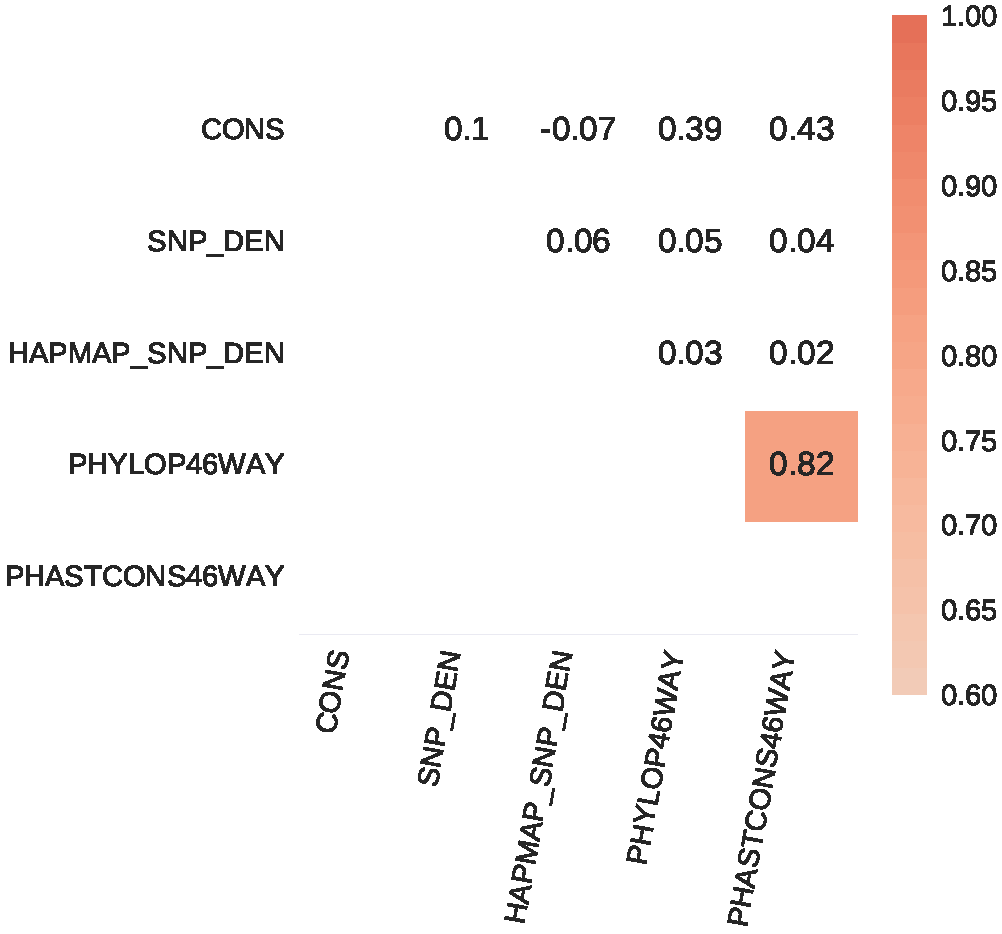
\includegraphics[scale=0.45]{documents/latex/figures/3/genomic/genomic_corr.pdf}
    \caption{Correlación de Spearman para las variables continuas del dataset Genómico.}
    \label{fig:corrplot_genomic}
\end{figure}

% \newpage

\section{Generación del modelo}

Luego de realizada la exploración del dataset Genómico generamos un modelo basado en Random Forest. Volvimos a utilizar este algoritmo debido a los resultados obtenidos en el dataset VarQ Curado y para facilitar la comparación entre los datasets estudiados. Volvimos a utilizar el Pipeline Tree descripto en el capítulo anterior. Nuevamente, las variables no fueron escaladas dado que en los algoritmos que involucran árboles de decisión, como Random Forest, las variables son evaluadas una a una y por lo tanto la escala de cada una de ellas no afecta la evaluación de las demás.

\section{Resultados del modelo Genómico}

Como se puede observar en la figura \ref{fig:auc_genomic} obtuvimos un AUC de 0.85. Los hiperparámetros escogidos en la fase de entrenamiento fueron una profundidad del árbol máxima (\texttt{max\_depth)} de 7, una cantidad máxima de variables de 7 (\texttt{max\_features}) y 100 estimadores (\texttt{\texttt{n\_estimators}}).
Este resultado es muy superior a los obtenidos en los modelos anteriores, tanto en VarQ Curado como en el dataset Físico-Químico. En la tabla \ref{tab:metrics_genomic} vemos los valores de Precision, Recall y F1-score para las dos clases. En este caso podemos advertir una mejora total en cada una de las métricas comparándolas con las obtenidas en base al modelo Físico-Químico. En particular destacamos la mejora en precisión de la detección de variables benignas, que pasó de un 0.68 en el modelo Físico-Químico a un 0.83 en el modelo Genómico, es decir un aproximadamente un 22\% de mejora; como así también el crecimiento en el Recall de variantes patogénicas, que saltó de un 0.47 en el modelo Físico-Químico a un 0.64, lo que representa casi un 36\% de mejora.

\begin{table}[H]
\centering
\begin{tabular}{|l|l|l|l|}
\hline
             & Precisión & Recall & F1-score \\ \hline
Benignas     & 0.83      & 0.87   & 0.85     \\ \hline
Patogénicas  & 0.69      & 0.64   & 0.67     \\ \hline
Promedio     & 0.79      & 0.79   & 0.79     \\ \hline
\end{tabular}
\caption{Reporte de métricas del modelo Random Forest usando el dataset Genómico.}
\label{tab:metrics_genomic}
\end{table}

% Otra de las razones que explican esta diferencia es la forma en que son calculadas. El dataset VarQ usa una variable basada a nivel de proteínas 


\section{Importancia de los atributos}
Analizando la importancia de las variables en el modelo, en la figura \ref{fig:importances_genomic} podemos observar que las variables de conservación (PHYLOP46WAY y PHASTCONS46WAY) están en los primeros dos puestos, confirmando lo obtenido por los trabajos de investigación antes mencionados \cite{Shihab2015} \cite{Carter2013} y su elevado AUC univariado. 

El poder informativo sumado de estas variables equivale a un porcentaje superior al 80\% de la importancia total. La pregunta que nos hacemos en este caso es: ¿Las dos primeras variables de conservación están en los primeros dos lugares porque están altamente correlacionadas o aportan diferente información sobre las variables? En base al análisis de correlación de Spearman (ver figura \ref{fig:corrplot_genomic}), podemos observar que estas variables se encuentran muy correlacionadas (0.82), lo que sugiere un alto grado de redundancia. En la figura \ref{fig:importance_genomic_cluster}, observamos que esta proporción se mantiene al agrupar en clusters a las variables correlacionadas.

Por otro lado, esto genera un interrogante adicional: ¿Cuál es la razón por la que la variable CONSERVATION del dataset VarQ Curado no genera un rendimiento similar? Una de las principales razones que encontramos es en el nivel de cobertura de la variable. En el caso de las variables de conservación genómica, la cobertura de las mismas llega a un nivel superior al 95\%, mientras que en el caso de la conservación en el dataset VarQ Curado este número no llega al 40\%. La cobertura de estas variables posee aproximadamente la misma proporción para variables patogénicas y benignas que la proporción original en ambos datasets. Otra razón posible a considerar tiene que ver con la naturaleza del cálculo de conservación de VarQ via PFAM, que contiene una heterogeneidad muy grande de especies (alrededor de 16,000 familias), y se basa en secuencias de proteínas, mientras que PHYLOP46WAY y PHASTCONS46WAY se basa en secuencias genómicas.

En resumen, hemos encontrado un modelo que supera en AUC ampliamente a los modelos anteriores. Sin embargo, no hay un salto significativo entre el AUC univariado (0.83 en PHYLOP46WAY) y el resultado final al combinar el resto de las variables y el algoritmo Random Forest. En el próximo capítulo evaluaremos la combinación de los datasets usando Humsavar y la posible mejora de un nuevo algoritmo, XGBoost.

\begin{figure}[H]
    \centering
    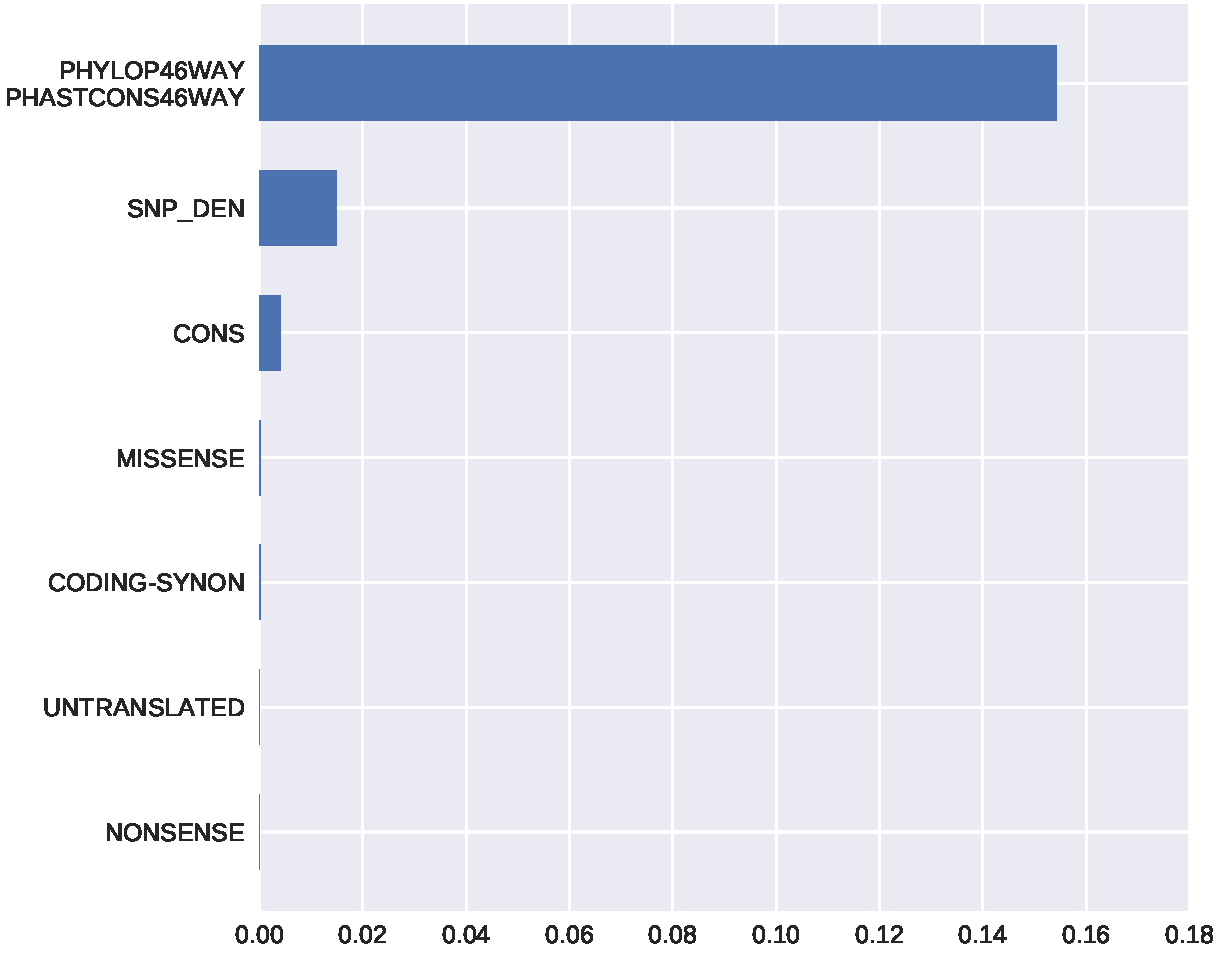
\includegraphics[scale=0.45]{documents/latex/figures/3/genomic/genomic_importance_cluster.pdf}
    \caption{Variación en el Accuracy al permutar clusters de variables correlacionadas (con un valor de correlación de Spearman superior a 0.60) del dataset Genómico.}
    \label{fig:importance_genomic_cluster}
\end{figure}

\newpage

\begin{figure}[H]
\centering
\begin{subfigure}[b]{0.7\textwidth}
    \centering
    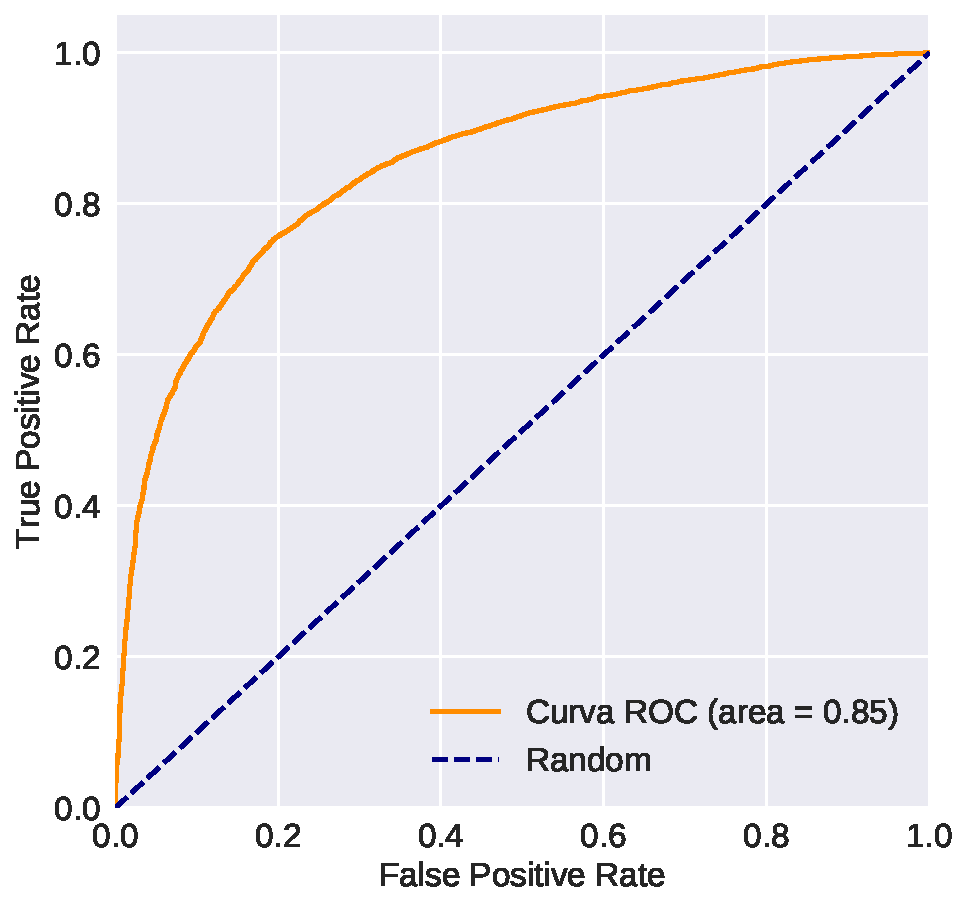
\includegraphics[width=\textwidth]{documents/latex/figures/3/genomic/auc_genomic.pdf}
    \caption{Curva AUC del modelo. La línea punteada corresponde a un predictor Random.}
    \label{fig:auc_genomic}
\end{subfigure}

\hfill
\hfill

\begin{subfigure}[b]{0.7\textwidth}
    \centering
    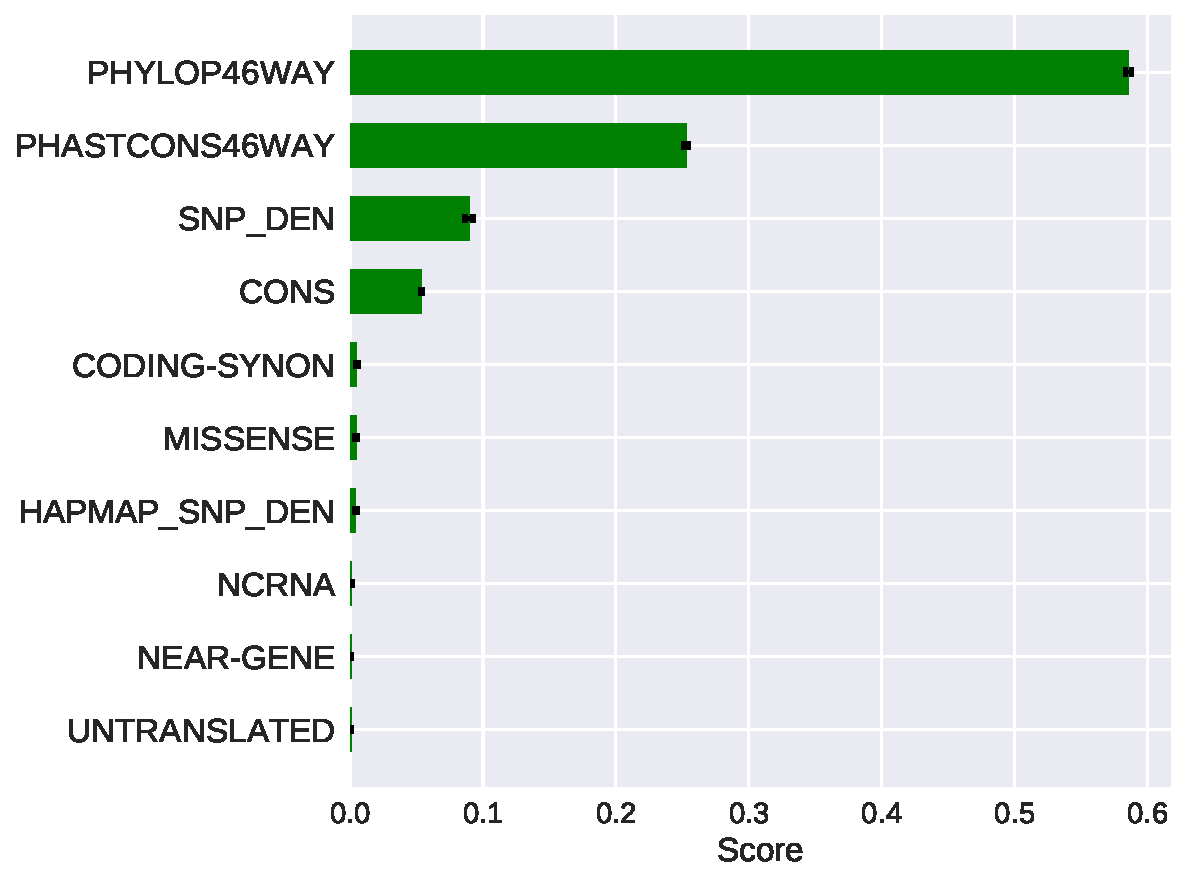
\includegraphics[width=\textwidth]{documents/latex/figures/3/genomic/importances_genomic.pdf}
    \caption{Los 10 atributos más importantes del modelo.}
    \label{fig:importances_genomic}
\end{subfigure}

\caption{Curva AUC y atributos más importantes del modelo Random Forest aplicado al dataset Genómico. Hiperparámetros del modelo: Profundidad del árbol 7, 7 variables en cada corte y 100 árboles.}

\end{figure}
